%!TeX root = ../index.tex

\section{Introduction}\label{sec:introduction}

\section{Reactive \acrlongpl{is}}

\citeauthor{boner_reactive_2014} describe how modern \glspl{is} of different domains all exhibit similar qualities.
\citetitle{boner_reactive_2014} summarizes those qualities and dubs the systems which feature them \enquote{reactive} \parencite{boner_reactive_2014}.
Put into the context of the quality dimensions defined by the \citetitle{iso_25010_2011} standard,
the reactive qualities cover only \enquote{Performance Efficiency} and \enquote{Reliability}.
While the other quality dimensions of the \citeauthor{iso_25010_2011} standard are certainly also important, this work focuses on the two mentioned before.

To quickly summarize \cite{boner_reactive_2014}, reactive systems are:

\begin{description}
  \item[Responsive] The system has low upper ceilings for its response times and meets these consistently.
  \item[Resilient] The system remains responsive in the face of failure.
  \item[Elastic] The system remains responsive under varying workload.
\end{description}

These qualities cover \enquote{reactive} systems from a technological perspective.
However, there is also a business perspective to the term.
Reactive systems also need to be flexible.
They need to be able to respond and change quickly according to changing requirements.
For example due to changing customer or market needs.
\citeauthor{beck2001agile} describe this quality as part of their \citetitle{beck2001agile} \parencite{beck2001agile}.
This work will refer to this quality as \emph{flexibility} from here on.

Different design and work patterns have emerged to create reactive systems.
One that is increasingly popular is microservice architecture \parencite{loukides_microservice_adoption_2020}.

\subsection{Microservice Architecture}

\citeauthor{richardson_microservices_2019} defines the microservice pattern as \enquote{an architectural style that functionally decomposes an application into a set of services} \parencite[11]{richardson_microservices_2019}.
The services are supposed to be loosely coupled, independently deployable, and scalable.
They are also small enough to be developed by a single, largely autonomous team.
The compartmentalization of the application also allows for it to tolerate partial failure.
If a single service fails, the rest of the application may stay partially functional.
\parencite[14f.]{richardson_microservices_2019}
These qualities contribute to the application's overall elasticity, resilience, and flexibility.

It is pointed out by \citeauthor{fowler_microservices_2014} that microservices commonly integrate with each other via synchronous communication protocols like \glspl{rpc} or HTTP \parencite{fowler_microservices_2014}.
This introduces different forms of coupling to the system.
First, the services need to know routes via which they can reach another directly.
Second, the services need to know not only the structure of the data they exchange but also the design anothers' \gls{api}.
Last, the synchronous nature of the communication couples the services in the dimension of time.
A service either completes a request in time, or the request reaches a timeout.
It is for this reason that many applications rely on asynchronous, message-driven communication via \gls{mom} \parencite{fowler_microservices_2014}.

\subsection{\acrlong{mom}}

\cite{boner_reactive_2014} defines one additional quality of reactive systems: message-driven.
Message-driven systems \enquote{rely on asynchronous message-passing to
establish a boundary between components that ensures loose coupling, isolation,
location transparency, and provides the means to delegate errors as messages.} \parencite{boner_reactive_2014}
As shown in figure \ref{fig:reactive-traits}, the message-driven quality actually forms the foundation for achieving all other qualities of a reactive system.

\begin{figure}
  \centering
  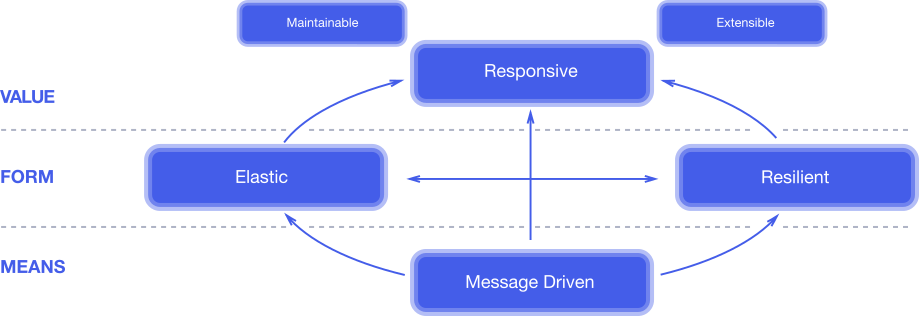
\includegraphics[width=\linewidth]{reactive-traits.png}
  \caption{The Qualities of a Reactive System \parencite{boner_reactive_2014}}
  \label{fig:reactive-traits}
\end{figure}

\cite{banavar_case_1999} coined the term of \acrlong{mom} for dedicated software components meant to integrate disparate applications in a distributed system by facilitating asynchronous message-passing between them.
\citeauthor{banavar_case_1999} based their work in part on the publish/subscribe semantics described in \cite{oki_information_1993} which are still present in the more comprehensive exploration of \gls{mom} in \cite{curry_message-oriented_2004} and prevail to this day.

There exist multiple established protocols which implement the patterns of \gls{mom} like AMQP and MQTT \parencites{amqp}{mqtt} and software solutions implementing the protocols (also called message brokers) like RabbitMQ or Mosquitto \parencites{rabbitmq}{mosquitto}.
While implementation details and terminology might vary between protocols and brokers, the general patterns are the same.

Clients \emph{publish} packets of data called \emph{messages} to a logical communication channel managed by the broker.
From here on, the text refers to such communication channels as \emph{topics}.
Clients can also \emph{subscribe} themselves to these topics and receive messages published to them.
Message delivery may be transient or persistent, meaning that messages are either delivered immediately to the subscribers of a topic by the broker or that the broker stores the messages in subscriber-specific, first-in-first-out queues.
Queues allow subscribers to consume messages at their own pace and become temporarily unavailable without losing messages.
\parencite{curry_message-oriented_2004}

However, one popular message broker does things a little differently.
The following section examines the ways in which Apache Kafka implements the patterns of \gls{mom}.

\subsection{Apache Kafka}

The LinkedIn employees \citeauthor{kreps_kafka_2011} introduced their new \enquote{Event Streaming Platform} \emph{Kafka} in \citeyear{kreps_kafka_2011} \parencite{kreps_kafka_2011}.
Over a decade later, the project has since joined the Apache foundation and \enquote{[m]ore than 80\% of all Fortune 100 companies trust, and use [it]} \parencite{apache_software_foundation_apache_nodate}.

\citeauthor{kreps_kafka_2011} describe Kafka as \enquote{[\ldots] a novel messaging system for log processing [\ldots] that combines the benefits of traditional log aggregators and messaging systems.} \parencite{kreps_kafka_2011}.
Similar to traditional \gls{mom}, \emph{producers} publish messages to logical communication channels called topics and \emph{consumers} can subscribe to topics to consume messages.
In contrast to traditional \gls{mom} however, topics are backed by one or more \emph{partitions}, an actual append-only data structure stored on the hard drive of a server running Kafka called a \emph{broker}.
Therefore, Kafka persists all messages sequentially for a configurable time even if the servers restart.
Partitions can also have replicas on other brokers, making Kafka tolerant against the failure of single servers.
A message in Kafka does not have a dedicated ID.
Instead, it is identified by its logical offset within its partition.
Consumers consume messages sequentially and move a pointer to the next offset after they have processed the message at the current position.
Furthermore, consumers can form groups in which no two members will subscribe to the same partition, thereby achieving a simple load balancing mechanism.
That also makes the number of partitions that a topic has the maximum degree of parallelism with which consumers can consume its messages.
\parencite{kreps_kafka_2011}

Kafka is not only useful for processing the kinds of log data that are proposed by \citeauthor{kreps_kafka_2011}: activity (e.~g. user logins, clicks, \enquote{likes}, \ldots) and operational data (e.~g. \gls{cpu} or disk utilization, HTTP requests, \ldots) \parencite{kreps_kafka_2011}.
\citeauthor{stopford_designing_2018}, for example, outlines how the entire state management and internal communication of a business application can be based on Apache Kafka.
His design implements concepts from the \gls{ddd} community like Event Sourcing \parencite{fowler_event_sourcing_2005} and \gls{cqrs} \parencite{fowler_cqrs_2011} with Apache Kafka's log-based messaging at the center \parencite{stopford_designing_2018}.
The potential use cases of Apache Kafka are therefore plentiful.

\section{Schemas}

\subsection{Schema Evolution}

\subsection{Schema Revolution}

\subsection{Apache Avro}

Apache Avro provides the ability to define rich data structures and interfaces for \glspl{rpc} as schema documents.
On top of that, it offers an efficient binary data format for serialization.
Listing \ref{lst:avro-schema-person} shows an example for an Avro schema describing a customer entity.
\parencite{apache_software_foundation_apache_2021}

\begin{listing}[H]
  \inputminted{json}{assets/src/Customer.avsc}
  \caption{Simplified Avro Schema of a Customer Entity}\label{lst:avro-schema-person}
\end{listing}

Avro's design assumes that applications which (de-)serialize data have access to the data's schema.
That is one of the reasons why the format is so efficient.
It does not need to include type information in the serialized data.
Avro's support for schema evolution builds upon this assumption.
If an application attempts to de-serialize data encoded in Avro binary, it requires both the schema with which the data was written and the schema which the application understands.
These schemas are called the \emph{writer} and the \emph{reader} schema respectively.
In the simplest case, these schemas might be equal.
Nevertheless, Avro also supports de-serializing data with a reader schema different from the writer schema.
Although, the de-serialization will only succeed if both schemas are still \emph{compatible}.
\parencite{apache_software_foundation_apache_2021}

If, for example, the reader schema had an additional field without a default value.
It would be an incompatible change because Avro would not be able to infer a value for the additional field.
On the other hand, if the field had a default value, the de-serialization would succeed.
\citeauthor{kreps_kafka_2011} chose Apache Avro as the serialization protocol for their message payloads due to its efficiency and schema evolution capabilities \parencite{kreps_kafka_2011}. 

\section{Schema Management}

\subsection{Schemas in Distributed Systems}

\subsection{Schema Management Solutions}

\section{Overview of Schema Management Solutions}
